% Options for packages loaded elsewhere
\PassOptionsToPackage{unicode}{hyperref}
\PassOptionsToPackage{hyphens}{url}
%
\documentclass[
  letterpaper,
]{book}

\usepackage{amsmath,amssymb}
\usepackage{iftex}
\ifPDFTeX
  \usepackage[T1]{fontenc}
  \usepackage[utf8]{inputenc}
  \usepackage{textcomp} % provide euro and other symbols
\else % if luatex or xetex
  \usepackage{unicode-math}
  \defaultfontfeatures{Scale=MatchLowercase}
  \defaultfontfeatures[\rmfamily]{Ligatures=TeX,Scale=1}
\fi
\usepackage{lmodern}
\ifPDFTeX\else  
    % xetex/luatex font selection
\fi
% Use upquote if available, for straight quotes in verbatim environments
\IfFileExists{upquote.sty}{\usepackage{upquote}}{}
\IfFileExists{microtype.sty}{% use microtype if available
  \usepackage[]{microtype}
  \UseMicrotypeSet[protrusion]{basicmath} % disable protrusion for tt fonts
}{}
\makeatletter
\@ifundefined{KOMAClassName}{% if non-KOMA class
  \IfFileExists{parskip.sty}{%
    \usepackage{parskip}
  }{% else
    \setlength{\parindent}{0pt}
    \setlength{\parskip}{6pt plus 2pt minus 1pt}}
}{% if KOMA class
  \KOMAoptions{parskip=half}}
\makeatother
\usepackage{xcolor}
\setlength{\emergencystretch}{3em} % prevent overfull lines
\setcounter{secnumdepth}{5}
% Make \paragraph and \subparagraph free-standing
\ifx\paragraph\undefined\else
  \let\oldparagraph\paragraph
  \renewcommand{\paragraph}[1]{\oldparagraph{#1}\mbox{}}
\fi
\ifx\subparagraph\undefined\else
  \let\oldsubparagraph\subparagraph
  \renewcommand{\subparagraph}[1]{\oldsubparagraph{#1}\mbox{}}
\fi


\providecommand{\tightlist}{%
  \setlength{\itemsep}{0pt}\setlength{\parskip}{0pt}}\usepackage{longtable,booktabs,array}
\usepackage{calc} % for calculating minipage widths
% Correct order of tables after \paragraph or \subparagraph
\usepackage{etoolbox}
\makeatletter
\patchcmd\longtable{\par}{\if@noskipsec\mbox{}\fi\par}{}{}
\makeatother
% Allow footnotes in longtable head/foot
\IfFileExists{footnotehyper.sty}{\usepackage{footnotehyper}}{\usepackage{footnote}}
\makesavenoteenv{longtable}
\usepackage{graphicx}
\makeatletter
\def\maxwidth{\ifdim\Gin@nat@width>\linewidth\linewidth\else\Gin@nat@width\fi}
\def\maxheight{\ifdim\Gin@nat@height>\textheight\textheight\else\Gin@nat@height\fi}
\makeatother
% Scale images if necessary, so that they will not overflow the page
% margins by default, and it is still possible to overwrite the defaults
% using explicit options in \includegraphics[width, height, ...]{}
\setkeys{Gin}{width=\maxwidth,height=\maxheight,keepaspectratio}
% Set default figure placement to htbp
\makeatletter
\def\fps@figure{htbp}
\makeatother

\makeatletter
\@ifpackageloaded{bookmark}{}{\usepackage{bookmark}}
\makeatother
\makeatletter
\@ifpackageloaded{caption}{}{\usepackage{caption}}
\AtBeginDocument{%
\ifdefined\contentsname
  \renewcommand*\contentsname{Table of contents}
\else
  \newcommand\contentsname{Table of contents}
\fi
\ifdefined\listfigurename
  \renewcommand*\listfigurename{List of Figures}
\else
  \newcommand\listfigurename{List of Figures}
\fi
\ifdefined\listtablename
  \renewcommand*\listtablename{List of Tables}
\else
  \newcommand\listtablename{List of Tables}
\fi
\ifdefined\figurename
  \renewcommand*\figurename{Figure}
\else
  \newcommand\figurename{Figure}
\fi
\ifdefined\tablename
  \renewcommand*\tablename{Table}
\else
  \newcommand\tablename{Table}
\fi
}
\@ifpackageloaded{float}{}{\usepackage{float}}
\floatstyle{ruled}
\@ifundefined{c@chapter}{\newfloat{codelisting}{h}{lop}}{\newfloat{codelisting}{h}{lop}[chapter]}
\floatname{codelisting}{Listing}
\newcommand*\listoflistings{\listof{codelisting}{List of Listings}}
\makeatother
\makeatletter
\makeatother
\makeatletter
\@ifpackageloaded{caption}{}{\usepackage{caption}}
\@ifpackageloaded{subcaption}{}{\usepackage{subcaption}}
\makeatother
\ifLuaTeX
  \usepackage{selnolig}  % disable illegal ligatures
\fi
\usepackage{bookmark}

\IfFileExists{xurl.sty}{\usepackage{xurl}}{} % add URL line breaks if available
\urlstyle{same} % disable monospaced font for URLs
\hypersetup{
  pdftitle={Die Tafelstube},
  pdfauthor={Lena-Marie Hoppe},
  hidelinks,
  pdfcreator={LaTeX via pandoc}}

\title{Die Tafelstube}
\author{Lena-Marie Hoppe}
\date{2024-05-31}

\begin{document}
\frontmatter
\maketitle

\renewcommand*\contentsname{Table of contents}
{
\setcounter{tocdepth}{2}
\tableofcontents
}
\mainmatter
\bookmarksetup{startatroot}

\chapter{Katalog zur Ausstellung: Die Tafelstube (Belangerungsszenden
des Langen Türkenkriegs an der
Decke)}\label{katalog-zur-ausstellung-die-tafelstube-belangerungsszenden-des-langen-tuxfcrkenkriegs-an-der-decke}

Ein Katalog mit Kunstwerken aus der CbDD-Sammlung. Textteil:
\href{https://www.deckenmalerei.eu/42d06165-58e7-4653-bfe4-3d5f7091fc33\#6e73f774-4b7f-4e37-937b-e11cc35c5bc8}{6e73f774-4b7f-4e37-937b-e11cc35c5bc8}

Die Tafelstube (Belagerungsszenen des Langen Türkenkriegs an der Decke)
{[}Raum{]}

This work is licensed under a Creative Commons
Attribution-NonCommercial-NoDerivs 4.0 International License.

\bookmarksetup{startatroot}

\chapter{Die Tafelstube}\label{die-tafelstube}

\textbf{How to use your own text for processing}

\begin{enumerate}
\def\labelenumi{\arabic{enumi}.}
\tightlist
\item
  Add a new Text item to the wikibase.
  \href{https://computational-publishing-service.wikibase.cloud/wiki/Special:NewItem}{link
  to wikibase new item} the item should contain the following
  statements:
\end{enumerate}

\begin{itemize}
\tightlist
\item
  P57 (external link): link to the html file containing the new text
\item
  P46 (kurator): Item of the curator. you may use an existing item like
  Q210 (Ulrike seeger) for test purposes
\item
  P53 (license): Item of a license for the text. e.g Q203 (CC BY-NC-ND
  4.0 DEED )
\item
  P6 (is part of): set value to Q218 (Schlossanlage Weikersheim)
\end{itemize}

\begin{enumerate}
\def\labelenumi{\arabic{enumi}.}
\setcounter{enumi}{1}
\item
  check if your new text item occurs in the list of selected text items:
  \href{https://computational-publishing-service.wikibase.cloud/query/\#PREFIX\%20cps\%3A\%20\%3Chttps\%3A\%2F\%2Fcomputational-publishing-service.wikibase.cloud\%2Fentity\%2F\%3E\%0APREFIX\%20cpss\%3A\%20\%3Chttps\%3A\%2F\%2Fcomputational-publishing-service.wikibase.cloud\%2Fentity\%2Fstatement\%2F\%3E\%0APREFIX\%20cpsv\%3A\%20\%3Chttps\%3A\%2F\%2Fcomputational-publishing-service.wikibase.cloud\%2Fvalue\%2F\%3E\%0APREFIX\%20cpspt\%3A\%20\%3Chttps\%3A\%2F\%2Fcomputational-publishing-service.wikibase.cloud\%2Fprop\%2Fdirect\%2F\%3E\%0APREFIX\%20cpsp\%3A\%20\%3Chttps\%3A\%2F\%2Fcomputational-publishing-service.wikibase.cloud\%2Fprop\%2F\%3E\%0APREFIX\%20cpsps\%3A\%20\%3Chttps\%3A\%2F\%2Fcomputational-publishing-service.wikibase.cloud\%2Fprop\%2Fstatement\%2F\%3E\%0APREFIX\%20cpspq\%3A\%20\%3Chttps\%3A\%2F\%2Fcomputational-publishing-service.wikibase.cloud\%2Fprop\%2Fqualifier\%2F\%3E\%0A\%0ASELECT\%20\%3FtextItem\%20\%3FkuratorLabel\%20\%3FtextUrl\%0AWHERE\%0A\%7B\%0A\%20\%20\%3FtextItem\%20cpsp\%3AP46\%20\%3FkuratorStatement.\%20\%0A\%20\%20\%3FkuratorStatement\%20cpsps\%3AP46\%20\%3FkuratorItem.\%20\%0A\%20\%20\%3FkuratorItem\%20rdfs\%3Alabel\%20\%3FkuratorLabel.\%0A\%20\%20\%3FtextItem\%20cpsp\%3AP57\%20\%3Furlstatement.\%20\%0A\%20\%20\%3Furlstatement\%20cpsps\%3AP57\%20\%3FtextUrl.\%20\%0A\%7D}{Link
  to wikibase query service}
\item
  set parameter of get\_text() to the id of your new text item e.g.:
  get\_text(``Q209'')
\end{enumerate}

Wikibase link:
\url{https://computational-publishing-service.wikibase.cloud/entity/Q232}

Kurator: Seeger, Ulrike

Die Tafelstube

Beschreibung

\xc3\x96stlich an den Rittersaal schlie\xc3\x9ft ein gro\xc3\x9fer, 1837
unterteilter Raum an, bei dem es sich um die einstige Tafelstube
handelt.{[}1{]} Als Eckraum mit vier Doppelfenstern zur Gartenseite und
weiteren drei Doppelfenstern zur Grabenseite erhielt die Tafelstube viel
Licht. Auch konnte der F\xc3\xbcrst von dort aus auf die Stadt und den
Lustgarten blicken, der in der Renaissance dem Schloss
s\xc3\xbcd\xc3\xb6stlich vorgelagert war.{[}2{]} Gemessen an der
Gr\xc3\xb6\xc3\x9fe des Raumes war die Tafelstube nicht sehr hoch. Die
Decke mit kr\xc3\xa4ftigen Unterz\xc3\xbcgen ruhte
urspr\xc3\xbcnglich auf vier St\xc3\xbctzen, deren Position einem Plan
des 19. Jahrhunderts zu entnehmen ist. Die Fensternischen waren in
Fortsetzung der Saaldekoration mit Roll- und Beschlagwerk stuckiert,
wof\xc3\xbcr Christoph Limmerich in Frage kommt, der auch im Saal
gearbeitet hat.

Logistisch geh\xc3\xb6ren zur Tafelstube zwei Service-Kabinetten
beiderseits des Durchgangs zwischen Saal und Tafelstube. Sie haben eine
geringe Raumh\xc3\xb6he, da \xc3\xbcber ihnen und dem Durchgang die
Empore an der Ostseite des Saals verl\xc3\xa4uft. Das Kabinett der
Gartenseite war von der Tafelstube und vom Durchgang aus
zug\xc3\xa4nglich, das Kabinett der Hofseite au\xc3\x9fer von der
Tafelstube vom Altan aus. Der Altan entlang der Hofseite des Saalbaus
verband das hofseitige Kabinett mit der K\xc3\xbcche im Erdgeschoss des
K\xc3\xbcchenbaus, sodass bevorzugt dieses Kabinett dem Anrichten der
Speisen gedient haben d\xc3\xbcrfte. Dank der Verbindung zu dem ja erst
in einem zweiten Bauabschnitt errichteten Altan, blieb der Rittersaal
vom Transport der Speisen verschont.

Der repr\xc3\xa4sentative Zugang zur Tafelstube erfolgte vom Saal aus,
wo der Besucher das imposante Portal mit der Belagerung von Gran
(Eszergom) im Hintergrund einer wilden T\xc3\xbcrkenschlacht,
bekr\xc3\xb6nt von der Skulptur des heiligen Georg zu durchschreiten
hatte. Ein zweiter Zugang bestand oder lie\xc3\x9f sich zumindest
einrichten von der geradel\xc3\xa4ufigen Treppe im sp\xc3\xa4teren
Langenburger Bau.

Die urspr\xc3\xbcngliche Bezeichnung des Raumes und seine Ausstattung

Im Inventar von 1625\xe2\x80\x9327 wurde der Raum im Anschluss an den
Saal als \xe2\x80\x9eSaalstube\xe2\x80\x9c bezeichnet.{[}3{]} Die
W\xc3\xa4nde waren mit 14 Ledertapeten beschlagen. Im Raum standen zwei
l\xc3\xa4ngsrechtecke Tische, ein quadratischer Tisch und eine
\xe2\x80\x9egro\xc3\x9fe Landtafel\xe2\x80\x9c sowie 31 Sessel mit
Lederbez\xc3\xbcgen und goldenem Dekor.{[}4{]} Im Schadensinventar von
1639 wurde der Raum sodann als \xe2\x80\x9eGro\xc3\x9fe
Tafelstube\xe2\x80\x9c gef\xc3\xbchrt.{[}5{]}

{[}1{]} Die Jahreszahl der Unterteilung: Merten, Weikersheim, o. J., S.
40; Fandrey, Weikersheim, 2010, S. 51.

{[}2{]} M\xc3\xbcnzenmayer/Elfgang, Schlossgarten, 1999, Abb. S. 5.

{[}3{]} Die Kenntnis dieses Inventars verdankt die Autorin Dinah
Rottsch\xc3\xa4fer.

{[}4{]} Ebd.

{[}5{]} HZAN La 130 B\xc3\xbc 152, Schadensinventar von 1639. Die
Kenntnis und die Transkription dieser Archivalie verdankt die Autorin
Frieder Leipold. Zur Herausbildung der Tafelstube im deutschen
Schlossbau der Renaissance: Hoppe, Tafelstube, 2007
(https://adw-goe.de/en/digital-library/hoefe-und-residenzen-im-spaetmittelalterlichen-reich/gsn/rf15\_II\_121207-196/?tx\_find\_find\%5BunderlyingQuery\%5D\%5Bq\%5D\%5Bdefault\%5D=tafelstube\&tx\_find\_find\%5BunderlyingQuery\%5D\%5Bposition\%5D=1)

\textbf{How to select images for processing}

Images are selected via the sparql query. The method get\_img() is
capable of using a wikibase item id as parameter to select images with
the property P6 (is part of) linking to the given item id.

\begin{enumerate}
\def\labelenumi{\arabic{enumi}.}
\item
  select a valid location id from the query result:
  \href{https://computational-publishing-service.wikibase.cloud/query/\#PREFIX\%20cps\%3A\%20\%3Chttps\%3A\%2F\%2Fcomputational-publishing-service.wikibase.cloud\%2Fentity\%2F\%3E\%0APREFIX\%20cpss\%3A\%20\%3Chttps\%3A\%2F\%2Fcomputational-publishing-service.wikibase.cloud\%2Fentity\%2Fstatement\%2F\%3E\%0APREFIX\%20cpsv\%3A\%20\%3Chttps\%3A\%2F\%2Fcomputational-publishing-service.wikibase.cloud\%2Fvalue\%2F\%3E\%0APREFIX\%20cpspt\%3A\%20\%3Chttps\%3A\%2F\%2Fcomputational-publishing-service.wikibase.cloud\%2Fprop\%2Fdirect\%2F\%3E\%0APREFIX\%20cpsp\%3A\%20\%3Chttps\%3A\%2F\%2Fcomputational-publishing-service.wikibase.cloud\%2Fprop\%2F\%3E\%0APREFIX\%20cpsps\%3A\%20\%3Chttps\%3A\%2F\%2Fcomputational-publishing-service.wikibase.cloud\%2Fprop\%2Fstatement\%2F\%3E\%0APREFIX\%20cpspq\%3A\%20\%3Chttps\%3A\%2F\%2Fcomputational-publishing-service.wikibase.cloud\%2Fprop\%2Fqualifier\%2F\%3E\%0A\%0ASELECT\%20DISTINCT\%20\%3FpartOfItem\%20\%3FpartOfItemLabel\%0AWHERE\%0A\%7B\%0A\%20\%20\%3FimgItem\%20cpsp\%3AP107\%20\%3FurlStatement.\%20\%0A\%20\%20\%3FurlStatement\%20cpsps\%3AP107\%20\%3FimgUrl.\%20\%0A\%20\%20\%3FimgItem\%20cpsp\%3AP60\%20\%3FdateStatement.\%20\%0A\%20\%20\%3FdateStatement\%20cpsps\%3AP60\%20\%3FpublishDate.\%20\%0A\%20\%20\%3FimgItem\%20cpsp\%3AP6\%20\%3FpartOfStatement.\%0A\%20\%20\%3FpartOfStatement\%20cpsps\%3AP6\%20\%3FpartOfItem.\%0A\%20\%20SERVICE\%20wikibase\%3Alabel\%20\%7B\%0A\%20\%20\%20\%20\%20\%20bd\%3AserviceParam\%20wikibase\%3Alanguage\%20\%22de\%2Cen\%22.\%0A\%20\%20\%20\%20\%20\%20\%3FpartOfItem\%20rdfs\%3Alabel\%20\%3FpartOfItemLabel.\%0A\%20\%20\%20\%20\%20\%20\%3FpartOfItem\%20schema\%3Adescription\%20\%3FpartOfItemDescr.\%0A\%20\%20\%20\%20\%7D\%0A\%7D\%20GROUP\%20BY\%20\%3FpartOfItem\%20\%3FpartOfItemLabel}{Link
  to wikibase query service}
\item
  set parameter of get\_img() to the id of your selected location item
  e.g.: get\_img(``Q217'')
\end{enumerate}

Wikibase link:
\url{https://computational-publishing-service.wikibase.cloud/entity/Q234}

Title: Einstige Tafelstube \& Raum 69a -- nach Südosten

Year: 2018

Description: Wolfgang Beringer, Baumeister und Steinmetz - Georg Stegle,
Baumeister - Entwurf: Georges Robin, Architekt - Elias Gunzenhäuser,
Zimmermann - Weikersheim, Marktplatz 11 - ab 1595

Wikibase link:
\url{https://computational-publishing-service.wikibase.cloud/entity/Q234}

Title: Einstige Tafelstube \& Raum 69a -- nach Südosten

Year: 2018-01-01T00:00:00Z

Description: Wolfgang Beringer, Baumeister und Steinmetz - Georg Stegle,
Baumeister - Entwurf: Georges Robin, Architekt - Elias Gunzenhäuser,
Zimmermann - Weikersheim, Marktplatz 11 - ab 1595

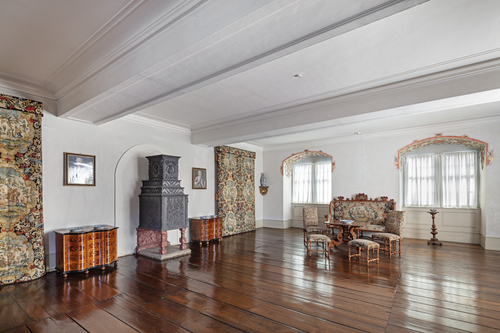
\includegraphics{section_files/figure-pdf/cell-4-output-2.png}
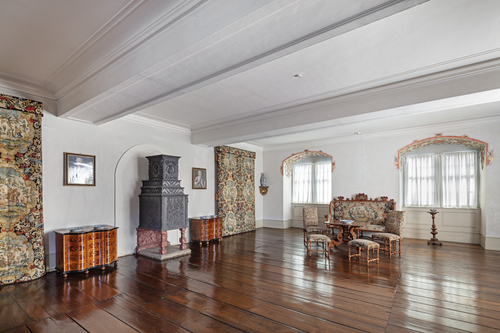
\includegraphics{section_files/figure-pdf/cell-4-output-3.png}

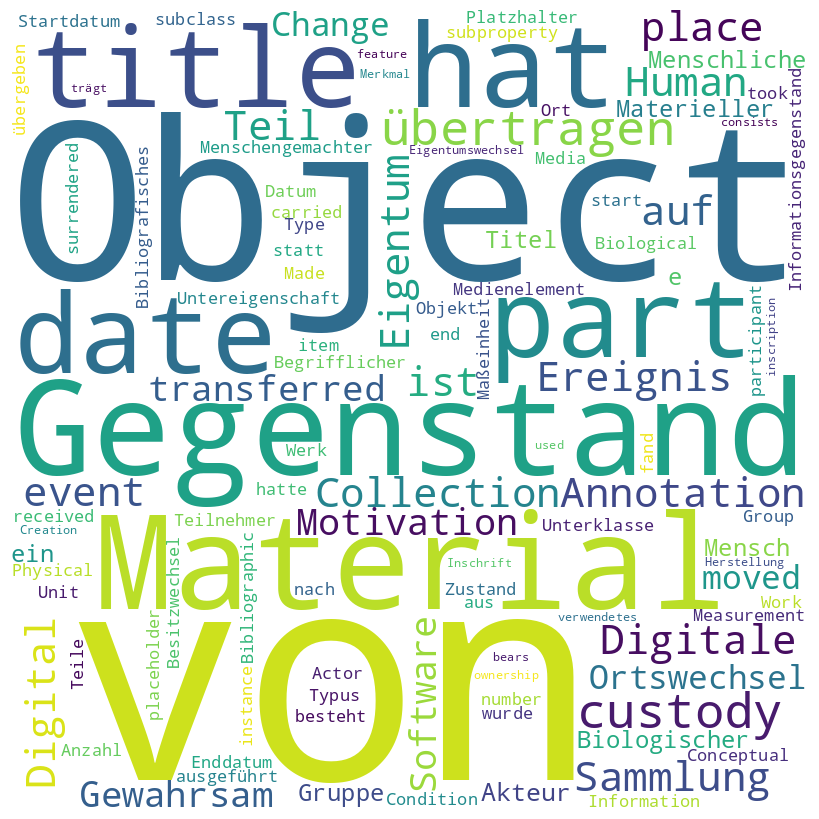
\includegraphics{section_files/figure-pdf/cell-5-output-1.png}


\backmatter

\end{document}
